\section{The central crossing at every \texorpdfstring{$N$}{N}}\label{sec:middle}

Let $N\ge2$, let $m_N=\lfloor N/2\rfloor$
and let $p>0$. By Theorem~\ref{thm:pmf} the ratio of the middle bin to an
endpoint is
\begin{equation}\label{eq:SN}
\frac{P_N(m_N)}{P_N(0)}=S_N(u):=\sum_{j=1}^{N-1}W(N,m_N,j)\,u^j ,
\end{equation}
a polynomial in $u$ with nonnegative integer coefficients and
$W(N,m_N,1)=2$. The middle and the endpoints are level exactly when
$S_N(u)=1$.

The following heuristic explains why this happens when $T$ is near $\log N$.
Let $a=m_N$ and
$b=N-m_N$, both about $N/2$. A word in the middle bin with $2r+1$ switches has
$r+1$ runs of each letter, and there are
$2\binom{a-1}r\binom{b-1}r\approx2(N/2)^{2r}/(r!)^2$ of them when $r$ is small
compared with $\sqrt N$. So these words contribute about
$2u\sum_r(Nu/2)^{2r}/(r!)^2=2uI_0(Nu)$ to $S_N(u)$, and in the same way the
words with an even number of switches contribute about $2uI_1(Nu)$. For large
$w=Nu$ we have $I_0(w)+I_1(w)\approx2e^w/\sqrt{2\pi w}$, so
$S_N(u)\approx4we^w/(N\sqrt{2\pi w})$. Setting this equal to $1$ gives
$w+\frac12\log w\approx L+\frac12\log(\pi/8)$. So at the crossing $w$, and with
it $T$, is close to $L-\frac12\log L+c_0$ with $c_0=\frac12\log(\pi/8)$.

\begin{theorem}\label{thm:root}
\begin{enumerate}[(a)]
\item For every $N\ge2$ there is exactly one $p=p_N\in[0,1]$ with
$P_N(m_N)=P_N(0)$, and $p_N\ge\tfrac23$. The middle is more likely than the
endpoints for $p<p_N$ and less likely for $p>p_N$.
\item $p_2=\tfrac23$, $p_3=1/\sqrt2$, $p_4$ is the real root of
$3p^3-4p^2+4p-2$, and $p_N<p_{N+1}$ for all $N\ge2$.
\item $p_N\to1$ as $N\to\infty$, and more precisely $1-p_N\sim(\log N)/N$.
\end{enumerate}
\end{theorem}

\begin{proof}
(a) At $p=0$ the endpoints have probability $0$ and the middle does not. For
$p>0$ the equation is $S_N(u)=1$ by \eqref{eq:SN}. The coefficients of $S_N$
are nonnegative and the linear one is $2$, so $S_N$ is strictly increasing on
$[0,\infty)$ with $S_N(0)=0$ and $S_N(u)\ge2u$. By the intermediate value
theorem there is exactly one root $u_N\in(0,\tfrac12]$. The map
$u\mapsto p=1/(1+u)$ is a decreasing bijection from $[0,\infty)$ to $(0,1]$.
Hence $p_N=1/(1+u_N)\ge\tfrac23$, and the middle wins exactly when $u>u_N$.

(b) By Theorem~\ref{thm:pmf}, $S_2=2u$, $S_3=2u+u^2$ and $S_4=2u+2u^2+2u^3$,
which give the three values. For $p_4$,
substitute $u=(1-p)/p$ in $S_4(u)=1$. For the monotonicity we compare
coefficients. Going from $N$ to $N+1$, one entry of the middle pair
$(a,b)=(\lfloor N/2\rfloor,\lceil N/2\rceil)$ grows by one and the other is
unchanged. The formulas of Theorem~\ref{thm:pmf} are symmetric in $(a,b)$, and
every $\binom{a-1}{\cdot}$ is nondecreasing in $a$. So
$W(N+1,m_{N+1},j)\ge W(N,m_N,j)$ for every $j$. The coefficient of $u^2$ is
$a+b-2=N-2$, which increases strictly. Hence $S_{N+1}(u)>S_N(u)$ for $u>0$, so
$u_{N+1}<u_N$.

(c) We prove (c) after Theorem~\ref{thm:bessel}, from part~(i) of that
theorem.
\end{proof}

In the tables of the problem, the middle and the endpoints of row $N+1$ are
level at $p=p_N$. The least value is $p_2=\tfrac23$ for the odd rows and
$p_3=1/\sqrt2$ for the even rows after the second (which is $1,1$ for every
$p$). There is no greatest value, since $p_N\uparrow1$. The tenth row has $p_9=0.82829\ldots$, just below
$\tfrac56$, so its middle and endpoints are nearly level in the third histogram of the
problem
(Figure~\ref{fig:row10} and Table~\ref{tab:pn}).

\begin{figure}[t]
\centering
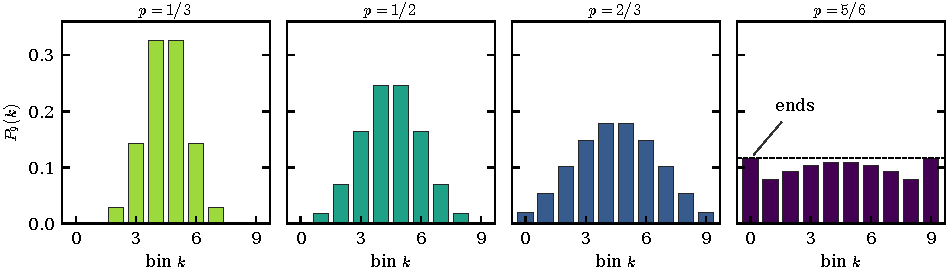
\includegraphics{figures/row10}
\caption{The bin probabilities $P_9(k)$ of the tenth row for
$p=\frac13,\frac12,\frac23,\frac56$. At $p=\frac56$, just above $p_9$, the two middle bins are
slightly below the endpoints (dashed line).}
\label{fig:row10}
\end{figure}

\begin{table}[ht]
\centering\small
\begin{tabular}{@{}rl@{\hskip 2em}rl@{\hskip 2em}rl@{\hskip 2em}rl@{}}
\toprule
$N$ & $p_N$ & $N$ & $p_N$ & $N$ & $p_N$ & $N$ & $p_N$\\
\midrule
2 & 0.66666667 & 6 & 0.78871211 & 10 & 0.83840411 & 50 & 0.94200405\\
3 & 0.70710678 & 7 & 0.80361731 & 11 & 0.84652725 & 100 & 0.96496633\\
4 & 0.74487450 & 8 & 0.81759938 & 12 & 0.85426060 & 200 & 0.97939018\\
5 & 0.76759188 & 9 & 0.82829163 & 20 & 0.89293837 & 400 & 0.98812464\\
\bottomrule
\end{tabular}
\caption{The value $p_N$ at which the middle and endpoint bins of row $N+1$ are equally likely.}
\label{tab:pn}
\end{table}

\subsection{A Bessel bound at every \texorpdfstring{$N$}{N}}

The heuristic above replaced the number $\binom{a-1}{r}$ of ways to split $a$
letters into $r+1$ runs by $a^r/r!$. After this change the run count is
exactly the power series of $I_0$ and $I_1$. The next lemma controls the error
of this change.

\begin{lemma}[clipped products]\label{lem:clipped}
(a) If $t_1,\dots,t_r\ge0$ and $(v)_+=\max(v,0)$, then
$0\le1-\prod_{k=1}^r(1-t_k)_+\le\sum_{k=1}^rt_k$.
(b) For integers $m\ge1$ and $r\ge0$,
$U_r(m):=\frac{r!}{m^r}\binom{m-1}{r}=\prod_{k=1}^r\bigl(1-\frac km\bigr)_+$,
so $0\le1-U_r(m)\le\frac{r(r+1)}{2m}$.
(c) For $x\ge0$,
\begin{gather*}
\sum_{r\ge0}\frac{r(r+1)x^{2r}}{(r!)^2}=x^2I_0(2x)+xI_1(2x),\\
\sum_{r\ge0}\frac{r(r+1)x^{2r+1}}{r!(r+1)!}=x^2I_1(2x),\qquad
\sum_{r\ge0}\frac{(r+1)x^{2r+1}}{r!(r+1)!}=xI_0(2x).
\end{gather*}
\end{lemma}

\begin{proof}
(a) Every factor lies in $[0,1]$, so the product is at most $1$. If some
$t_k\ge1$ the product is $0$ and the sum is at least $1$. Otherwise
$\prod_k(1-t_k)\ge1-\sum_kt_k$ by induction on $r$. (b) Note that
$\frac{r!}{m^r}\binom{m-1}{r}=\prod_{k=1}^r\frac{m-k}m$. For $r<m$ every factor
is positive, and for $r\ge m$ both sides vanish, the right side through the
factor $k=m$. The bound is (a) with $t_k=k/m$. (c) Use the series of $I_0(2x)$
and $I_1(2x)$ from Section~\ref{sec:setting}. Write $r(r+1)=r^2+r$ in the
first sum, cancel the factors $r$ and $r+1$ against the factorials, and shift
the index.
\end{proof}

\begin{theorem}[uniform Bessel approximation]\label{thm:bessel}
Put $h=N/2$ and $F(x)=2x\bigl(I_0(2x)+I_1(2x)\bigr)$, and recall that
$u_N=(1-p_N)/p_N$.
\begin{enumerate}[(i)]
\item For every $N\ge2$ and $x>0$,
\begin{equation}\label{eq:uniformbessel}
0\le1-\frac{hS_N(x/h)}{F(x)}\le\frac{x(x+1)}h.
\end{equation}
\item Let $x_N=hu_N$, let $x_B$ be the unique positive root of $F(x_B)=h$, and
put $\delta_N=x_N(x_N+1)/h$. Then $x_B\le x_N$, and
$x_N-x_B\le-\frac12\log(1-\delta_N)$ whenever $\delta_N<1$.
\item With $u_B=x_B/h$ we have $0\le u_N-u_B=O(L^2/N^2)$ as $N\to\infty$.
\end{enumerate}
\end{theorem}

Part~(i) holds at every $N\ge2$, and Section~\ref{sec:every-n-sub} uses it to
locate $p_N$ at every $N$.

\begin{proof}
(i) \emph{Step 1. The clipped factors.} Let $a=\lfloor N/2\rfloor$ and
$b=\lceil N/2\rceil$. As in Lemma~\ref{lem:clipped}(b),
$A_r=\frac{r!}{h^r}\binom{a-1}{r}=\prod_{k=1}^r(1-\frac{h-a+k}h)_+$, and $B_r$
is the same with $b$ in place of $a$. Since $a+b=2h$ and $h-a\in\{0,\frac12\}$,
the $2r$ numbers $(h-a+k)/h$ and $(h-b+k)/h$ are nonnegative with sum
$r(r+1)/h$, so Lemma~\ref{lem:clipped}(a) gives $0\le1-A_rB_r\le r(r+1)/h$. In
the same way the deficits of $A_{r+1}B_r$ and $A_rB_{r+1}$ are at most
$((r+1)^2+h-a)/h$ and $((r+1)^2+h-b)/h$. Averaging cancels the parity offsets,
so $0\le1-\frac12(A_{r+1}B_r+A_rB_{r+1})\le(r+1)^2/h$.

\emph{Step 2. Summing.} With $u=x/h$ the run-count formula of
Theorem~\ref{thm:pmf} becomes
\[
S_N(u)=2u\Bigl[\sum_{r\ge0}\frac{x^{2r}}{(r!)^2}A_rB_r
+\sum_{r\ge0}\frac{x^{2r+1}}{r!(r+1)!}\,\frac{A_{r+1}B_r+A_rB_{r+1}}2\Bigr].
\]
Without the factors $A_r,B_r$ the bracket is $I_0(2x)+I_1(2x)$ and the right
side is $F(x)/h$. By Step~1 and Lemma~\ref{lem:clipped}(c), $F(x)/h-S_N(u)$
lies between $0$ and $2u/h$ times
$\sum_rr(r+1)\frac{x^{2r}}{(r!)^2}+\sum_r(r+1)^2\frac{x^{2r+1}}{r!(r+1)!}=x(x+1)\bigl(I_0(2x)+I_1(2x)\bigr)$.
Dividing by $F(x)/h=2u(I_0(2x)+I_1(2x))$ proves (i). This covers every $r$,
also those beyond the degree of the polynomial, where the clipped products
vanish and Lemma~\ref{lem:clipped}(a) still applies.

(ii) Differentiating the series term by term gives $F'=2F+2I_0(2x)$. So $F$
increases from $0$ to $\infty$, $x_B$ is unique, and $(\log F)'\ge2$. At
$x=x_N$ we have $hS_N(u_N)=h$, so (i) gives $h\le F(x_N)$, hence $x_B\le x_N$,
and $F(x_N)\le h/(1-\delta_N)$ when $\delta_N<1$. Integrating $(\log F)'\ge2$
from $x_B$ to $x_N$ gives $2(x_N-x_B)\le\log(F(x_N)/h)\le-\log(1-\delta_N)$.

\emph{Proof of Theorem~\ref{thm:root}(c).} We use only part~(i). Note that
$x^{2r}/(r!)^2\le(2x)^{2r}/(2r)!$ and
$x^{2r+1}/(r!(r+1)!)\le(2x)^{2r+1}/(2r+1)!$ for $x\ge0$, since
$\binom{2r}r\le4^r$ and $\binom{2r+1}r\le2^{2r+1}$. So
$I_0(2x)+I_1(2x)\le e^{2x}$ and $F(x)\le2xe^{2x}$. Fix $\theta\in(0,1)$ and
put $x_\pm=(1\pm\theta)L/2$. Then $F(x_-)\le(1-\theta)LN^{1-\theta}<h$ for
large $N$, so $hS_N(x_-/h)<h$ by (i), and $x_-<x_N$ since $S_N$ increases. On
the other side $F(x_+)\ge2x_+I_0(2x_+)$, which is at least a constant times
$\sqrt L\,N^{1+\theta}$ for large $N$ by the large-argument form of $I_0$,
while $x_+(x_++1)/h\to0$. So $hS_N(x_+/h)\ge F(x_+)(1-x_+(x_++1)/h)>h$ for
large $N$, and $x_N<x_+$. Hence $Nu_N=2x_N\sim L$, so $u_N\to0$ and
$z_N=Nu_N/(1+u_N)\sim L$, which is (c).

(iii) By Theorem~\ref{thm:root}(c), $x_N\sim L/2$. So $\delta_N=O(L^2/N)$,
and (ii) gives $x_N-x_B=O(L^2/N)$. Divide by $h$.
\end{proof}

\subsection{The crossing at every \texorpdfstring{$N$}{N}}\label{sec:every-n-sub}

We measure the crossing by $z_N=N(1-p_N)=Nu_N/(1+u_N)$, the value of $T$ at
$p=p_N$. Let $\psi(z)=z+\frac12\log z$ and $c_0=\frac12\log(\pi/8)=-0.46735\ldots$,
and let $\zeta_N$ be the positive root of
\begin{equation}\label{eq:zetaN}
\psi(\zeta_N)=L+c_0,\quad\text{that is,}\quad 8\zeta_Ne^{2\zeta_N}=\pi N^2
\quad\text{or}\quad\zeta_N=\tfrac12W_0(\pi N^2/4),
\end{equation}
with $W_0$ the principal branch of the Lambert function. This is the
heuristic equation from the start of the section with $w$ replaced by $\zeta$.
Since $\zeta e^{2\zeta}$ increases, $\zeta_N$ increases with $N$. Also
$\zeta_N\le L$, since $\psi(L)\ge L+c_0$ when $L\ge\pi/8$. Finally let
$\varepsilon_N=\zeta_N(\zeta_N+1)/N+1/(16\zeta_N^2)$.

\begin{theorem}[the crossing at every $N$]\label{thm:every-n}
For every $N\ge2$,
\[
\zeta_N+\frac1{8\zeta_N}-\varepsilon_N<z_N<\zeta_N+\frac1{8\zeta_N}.
\]
\end{theorem}

The width $\varepsilon_N$ tends to $0$, since $\zeta_N\le L$ and
$\zeta_N\to\infty$. It is $0.440$, $0.163$, $0.0387$ and $0.00778$ at
$N=10,10^2,10^3,10^4$ (Table~\ref{tab:every-n}).

The two terms $\zeta_N$ and $1/(8\zeta_N)$ come from the following heuristic.
Let
$\Phi(w)=F(w/2)=w\bigl(I_0(w)+I_1(w)\bigr)$ and
$\cE(z)=\sqrt{\pi z/2}\,e^{-z}\bigl(I_0(z)+I_1(z)\bigr)$, which tends to $1$ as
$z\to\infty$. Put $w_N=Nu_N$ and $\Lambda_N=2\Phi(w_N)/N$. At the crossing,
\eqref{eq:uniformbessel} and \eqref{eq:bracket-log} below give
$\psi(w_N)+\log \cE(w_N)=L+c_0+\log\Lambda_N$ with
$0\le\log\Lambda_N\le-\log(1-w_N(w_N+2)/(2N))$. With $\cE=\Lambda_N=1$ this
would say $w_N=\zeta_N$. Since $\log \cE(w)=-1/(8w)+O(w^{-2})$ and
$z_N=w_N+O(w_N^2/N)$, it suggests
$z_N=\zeta_N+1/(8\zeta_N)+O(\zeta_N^{-2}+\zeta_N^2/N)$. The theorem makes this
error explicit and one-sided. Its proof uses two lemmas. Lemma~\ref{lem:bracket}
turns a comparison of $z_N$ with a test value into a sign condition, and
Lemma~\ref{lem:bessel-bounds} bounds $\cE$ with explicit constants.

\begin{lemma}[root bracket]\label{lem:bracket}
Let $N\ge2$ and $w>0$. Then
\begin{equation}\label{eq:bracket-log}
\log\Phi(w)-\log\tfrac N2=\psi(w)-\psi(\zeta_N)+\log \cE(w).
\end{equation}
(a) If $\Phi(w)\le N/2$, then $Nw/(N+w)\le z_N$, strictly if $\Phi(w)<N/2$.
(b) If $\Phi(w)\bigl(1-\frac{w(w+2)}{2N}\bigr)>N/2$, then $z_N<Nw/(N+w)$.
\end{lemma}

\begin{proof}
Note that $\log\Phi(w)=\psi(w)+\frac12\log\frac2\pi+\log \cE(w)$ and
$\log\frac N2-\psi(\zeta_N)=-\log2-c_0=\frac12\log\frac2\pi$, which gives
\eqref{eq:bracket-log}. Now apply \eqref{eq:uniformbessel} with $x=w/2$. Then
$F(x)=\Phi(w)$ and $x(x+1)/h=w(w+2)/(2N)$, so
\[
\Phi(w)\Bigl(1-\frac{w(w+2)}{2N}\Bigr)\le\frac N2\,S_N\Bigl(\frac wN\Bigr)\le\Phi(w).
\]
(a) The hypothesis gives $S_N(w/N)\le1=S_N(u_N)$, strictly if $\Phi(w)<N/2$.
Since $S_N$ is strictly increasing, $w/N\le u_N$, strictly in that case. The
map $v\mapsto Nv/(1+v)$ increases and sends $w/N$ to $Nw/(N+w)$ and $u_N$ to
$z_N$. (b) Now $S_N(w/N)>1$, so $w/N>u_N$.
\end{proof}

\begin{lemma}[Bessel bounds]\label{lem:bessel-bounds}
For every $z>0$,
\[
1-\frac1{8z}-\frac3{128z^2}-\frac{45}{512z^3}\le \cE(z)\le1-\frac1{8z}-\frac3{128z^2}+\frac{15}{512z^3},
\]
and $\cE(z)\le1$. In particular $\cE(z)\le1-\frac1{8z}$ for $z\ge\frac54$.
\end{lemma}

The lemma is the large-argument expansion of $I_0+I_1$ with explicit errors.
We prove it in Appendix~\ref{app:every-n}. By \cite[Eq.~10.32.3]{dlmf} and a
substitution,
$\cE(z)=\pi^{-1/2}\int_0^{2z}e^{-v}v^{-1/2}\sqrt{1-v/(2z)}\,dv$. We bound
$\sqrt{1-y}$ above and below by cubics that share its Taylor terms up to $y^2$,
extend the integral to $\infty$, and use
$\Gamma(k+\frac12)/\Gamma(\frac12)=1,\frac12,\frac34,\frac{15}8$ for
$k=0,1,2,3$.

\begin{proof}[Proof of Theorem~\ref{thm:every-n}]
\emph{Step 1. The split at $N=175$.} By \eqref{eq:zetaN},
$N=\sqrt{8\zeta_N/\pi}\,e^{\zeta_N}$, and the right side increases in
$\zeta_N$. Since $\sqrt{32/\pi}\,e^4=174.25\ldots$, we have $\zeta_N\ge4$
exactly when $N\ge175$. Write $\zeta=\zeta_N$ and $U=\zeta+\frac1{8\zeta}$.

\emph{Step 2. The upper bound for $N\ge175$.} We apply
Lemma~\ref{lem:bracket}(b) at $W=NU/(N-U)$, for which $NW/(N+W)=U$. By
\eqref{eq:bracket-log} it suffices that
$G_U=\psi(W)-\psi(\zeta)+\log \cE(W)+\log(1-W(W+2)/(2N))>0$. Expanding each
term with Lemma~\ref{lem:bessel-bounds} gives
$G_U\ge\frac1{32\zeta^2}+\frac{\zeta(\zeta-1)}{2N}+O(\zeta^{-3}+N^{-1}+\zeta^4N^{-2})$,
and Appendix~\ref{app:every-n} makes every term explicit for $\zeta\ge4$.

\emph{Step 3. The lower bound for $N\ge175$.} We apply
Lemma~\ref{lem:bracket}(a) at $W'=NU'/(N-U')$ with
$U'=U-\varepsilon_N$. It suffices that
$G_{U'}=\psi(W')-\psi(\zeta)+\log \cE(W')<0$, and we get
$G_{U'}\le-\frac3{128\zeta^2}-\frac\zeta N+O(\zeta^{-3}+N^{-1}+\zeta^4N^{-2})$,
again with explicit constants for every $\zeta\ge4$ in
Appendix~\ref{app:every-n}. The term $-\zeta/N$ is why $\varepsilon_N$
contains $\zeta(\zeta+1)/N$.

\emph{Step 4. $2\le N\le174$, by certificates.} Let $d=10^9$ and let $c<c'$ be
integers with $c'=c+1$ ($c'=c+2$ at $N=2$, where $u_2=\frac12$ is a grid
point). The sign of $S_N(c/d)-1$ is the sign of $n_N(m_N)-d^{N-1}$, where
$n_N(m_N)=d^{N-1}S_N(c/d)$ is the integer of Remark~\ref{rem:tables} at
$(\alpha,\beta)=(d,c)$ (Appendix~\ref{app:certificates}). We computed these
integers at $c$ and $c'$ by two exact methods, the run-count sum of
Theorem~\ref{thm:pmf} and the recursion \eqref{eq:dp} with integer weights
$d,c$ in place of $p,q$. They agreed for every $N\le174$ and gave
$c/d<u_N<c'/d$, so $z(c/d)<z_N<z(c'/d)$ with $z(u)=Nu/(1+u)$. We then checked
$\zeta_N+\frac1{8\zeta_N}-\varepsilon_N<z(c/d)$ and
$z(c'/d)<\zeta_N+\frac1{8\zeta_N}$ in 60-digit decimal arithmetic, with
$\zeta_N$ in a bracket of width $10^{-45}$. We certified this bracket by the
sign of $\psi(\zeta)-L-c_0$, which is the sign of $8\zeta e^{2\zeta}-\pi N^2$,
at both of its ends, using a correctly rounded logarithm. The smallest margins
are $0.033193$ (upper) and $0.085591$ (lower), both at $N=174$. Rounding cannot change these comparisons. Put
$g_1(\zeta)=\zeta+\frac1{8\zeta}$ and
$g_2(\zeta)=g_1(\zeta)-\frac{\zeta(\zeta+1)}N-\frac1{16\zeta^2}$. For
$\frac12\le\zeta\le L+1$ and $N\ge2$ we have $|g_1'|,|g_2'|\le5$, and
$\frac12<\zeta_2\le\zeta_N\le L$. So $g_1$ and $g_2$ vary by at most
$5\cdot10^{-45}$ on the bracket, and the decimal evaluation adds at most
$10^{-50}$. Both are far below the margin $0.03$. The Lean proof checks the same
comparisons with rational bounds on $\zeta_N$ and $\pi$. As a cross-check, the
certificates also pass for $N\le1000$, by both methods up to $400$ and by the
run-count sum after that.
\end{proof}

\begin{table}[ht]
\centering\small
\begin{tabular}{@{}rllrrr@{}}
\toprule
$N$ & $z_N$ & $\zeta_N$ & $z_N-\zeta_N-\frac1{8\zeta_N}$ & $-\varepsilon_N$ & $R_N$\\
\midrule
2 & 0.666666666667 & 0.5368290974 & $-0.1030112$ & $-0.62938$ & $+0.050643$\\
10 & 1.615958871376 & 1.6001732978 & $-0.0623310$ & $-0.44048$ & $-0.056660$\\
100 & 3.503367368092 & 3.5100055489 & $-0.0422507$ & $-0.16337$ & $-0.043265$\\
174 & 3.996779704730 & 3.9987131703 & $-0.0331935$ & $-0.11878$ & $-0.033450$\\
175 & 4.001967989170 & 4.0038072816 & $-0.0330596$ & $-0.11838$ & $-0.033304$\\
1000 & 5.590351166975 & 5.5807388611 & $-0.0127862$ & $-0.03873$ & $-0.011887$\\
$10^4$ & 7.734265514999 & 7.7210118331 & $-0.0029359$ & $-0.00778$ & $-0.002051$\\
\bottomrule
\end{tabular}
\caption{The crossing against Theorem~\ref{thm:every-n}, and the remainder $R_N$ of
\eqref{eq:crossing-eq}. We computed $z_N$ by run-count bisection in 60-digit decimal arithmetic
and by a floating-point dynamic program, which agree to the digits shown.}
\label{tab:every-n}
\end{table}

The bracket involves $\zeta_N$. The next corollary states it for $p_N$ and
expands it in $L=\log N$.

\begin{corollary}\label{cor:every-n}
Put $\nu_N=L-\frac12\log L+c_0$.
\begin{enumerate}[(a)]
\item For every $N\ge2$,
$1-\bigl(\zeta_N+\frac1{8\zeta_N}\bigr)/N<p_N<1-\bigl(\zeta_N+\frac1{8\zeta_N}-\varepsilon_N\bigr)/N$.
\item For every $N\ge2$, $\nu_N\le\zeta_N\le\nu_N+\frac{\log L-2c_0}{4\nu_N}$ and
\begin{equation}\label{eq:secondorder}
-\varepsilon_N<z_N-\nu_N<\frac{\log L-2c_0+\frac12}{4\nu_N}.
\end{equation}
In particular $z_N=L-\frac12\log L+c_0+O(\log L/L)$ as $N\to\infty$.
\item As $N\to\infty$,
\begin{equation}\label{eq:thirdorder}
z_N=\nu_N+\frac{\frac14\log L-\frac12c_0+\frac18}{L}+O\Bigl(\frac{(\log L)^2}{L^2}\Bigr).
\end{equation}
\item (Computer-assisted.) $z_N>\zeta_N$ for every $N\ge2774$.
\end{enumerate}
\end{corollary}

\begin{proof}
(a) is Theorem~\ref{thm:every-n} with $p_N=1-z_N/N$.

(b) By \eqref{eq:zetaN}, $\zeta_N=L+c_0-\frac12\log\zeta_N$. Since
$\zeta_N\le L$, this gives $\zeta_N\ge\nu_N$, and $\nu_N>0$ since it increases
in $N$ and $\nu_2=0.41$. Also $\log y\le y-1$ gives
$\zeta_N-\nu_N=\frac12\log(L/\zeta_N)\le(L-\zeta_N)/(2\zeta_N)$, and
$L-\zeta_N=\frac12\log\zeta_N-c_0\le\frac12\log L-c_0$. Hence
$\zeta_N-\nu_N\le(\log L-2c_0)/(4\nu_N)$. For $z_N$, add
Theorem~\ref{thm:every-n} and $0<\frac1{8\zeta_N}\le\frac1{8\nu_N}$. The last
claim follows since $\varepsilon_N=O(L^2/N+L^{-2})$.

(c) Put $\eta=\zeta_N-\nu_N=\frac12\log(L/\zeta_N)$. By (b),
$L-\zeta_N=\frac12\log L-c_0+O(\log L/L)$, so
$\eta=\frac{L-\zeta_N}{2L}+O\bigl(\frac{(\log L)^2}{L^2}\bigr)
=\frac{\frac14\log L-\frac12c_0}L+O\bigl(\frac{(\log L)^2}{L^2}\bigr)$.
Also $\frac1{8\zeta_N}=\frac1{8L}+O(\frac{\log L}{L^2})$ and
$\varepsilon_N=O(L^2/N+L^{-2})$, and Theorem~\ref{thm:every-n} gives (c).

(d) By Theorem~\ref{thm:every-n}, $z_N-\zeta_N>\frac1{8\zeta_N}-\varepsilon_N$,
which is positive when $f(\zeta_N)>1$, where
$f(\zeta)=n(\zeta)\bigl(\frac1{8\zeta}-\frac1{16\zeta^2}\bigr)/(\zeta(\zeta+1))$
and $n(\zeta)=\sqrt{8\zeta/\pi}\,e^\zeta$, so that $n(\zeta_N)=N$. The
logarithmic derivative of $f$ is
$1+\frac1{2\zeta}-\frac2\zeta+\frac1{2\zeta^2-\zeta}-\frac1{\zeta+1}>1-\frac3{2\zeta}-\frac1{\zeta+1}>0$
for $\zeta\ge3$. Since $\zeta_N$ increases with $N$, once $f(\zeta_N)>1$ it
stays above $1$. This step is computer-assisted. In 60-digit decimal
arithmetic, with $\zeta_N$ bracketed within $10^{-45}$ as in Step~4 above, we
found $f(\zeta_{2774})-1=2.1\times10^{-4}$, and the sign holds on the whole
bracket. Since $\zeta_{2774}>3$, this proves (d). The condition fails at $N=2773$.
\end{proof}

The heuristic suggests that $\psi(z_N)\approx L+c_0+1/(8z_N)$. The next
proposition proves this at every $N$ with an explicit remainder.

\begin{proposition}[the crossing equation]\label{prop:crossing-eq}
For every $N\ge2$,
\begin{equation}\label{eq:crossing-eq}
z_N+\tfrac12\log z_N=L+c_0+\frac1{8z_N}+R_N,\qquad
-\frac{z_N^2+z_N}N\le R_N\le\frac1{16z_N^2}.
\end{equation}
Moreover $L/2\le z_N\le L$, so $|R_N|\le\frac1{4L^2}+\frac{L^2+L}N$ for every
$N\ge2$.
\end{proposition}

We prove Proposition~\ref{prop:crossing-eq} in Appendix~\ref{app:every-n}.
The proof writes $R_N$ exactly, using \eqref{eq:uniformbessel} and
\eqref{eq:bracket-log} at $w=w_N$ (formula \eqref{eq:RN-formula}). For
$N\ge175$, Lemma~\ref{lem:bessel-bounds} puts the Bessel part of this formula
between $0$ and $0.0559/z_N^2$, and the other terms lie between
$-(z_N^2+z_N)/N$ and $0$. For $N\le174$ the proof uses the same certificates as
Theorem~\ref{thm:every-n}.

\begin{remark}[the sign of $z_N-\zeta_N$, computer-assisted]\label{rem:sign}
We have $z_N>\zeta_N$ for $N\le15$, $z_N<\zeta_N$ for $16\le N\le218$, and
$z_N>\zeta_N$ for every $N\ge219$. For $N\le1000$ the certificates decide the
sign, since $\zeta_N$ never lies in $[z(c/d),z(c'/d)]$. The smallest distance
is $1.66\times10^{-5}$, at $N=218$. Both exact methods cover $N\le400$, and the
run-count sum alone covers the rest. For $1001\le N\le2773$ we checked
$S_N(v)<1$ in exact integers from the run-count sum, at a rational $v$ above
$\zeta_N/(N-\zeta_N)$ by at least $1.2\times10^{-11}$, where
$z(\zeta_N/(N-\zeta_N))=\zeta_N$. These integers were cross-checked by
floating-point run-count and dynamic-program sign tests for every $N\le3000$,
and by the integer recursion at $N=401,1000,1008,2000,2773$. For $N\ge2774$
the sign is Corollary~\ref{cor:every-n}(d).
\end{remark}

The ratios $u_B/u_N$ of the Bessel root of Theorem~\ref{thm:bessel} to the
true odds are $0.9761$, $0.9864$,
$0.9924$ at $N=100,200,400$ and $0.99579$, $0.99769$, $0.99874$ at
$N=800,1600,3200$, in line with the relative error $O(L^2/N)$ of
Theorem~\ref{thm:bessel}. Figure~\ref{fig:crossing} compares the exact crossing
with the expansions of Corollary~\ref{cor:every-n} up to $N=10^4$.

\begin{figure}[t]
\centering
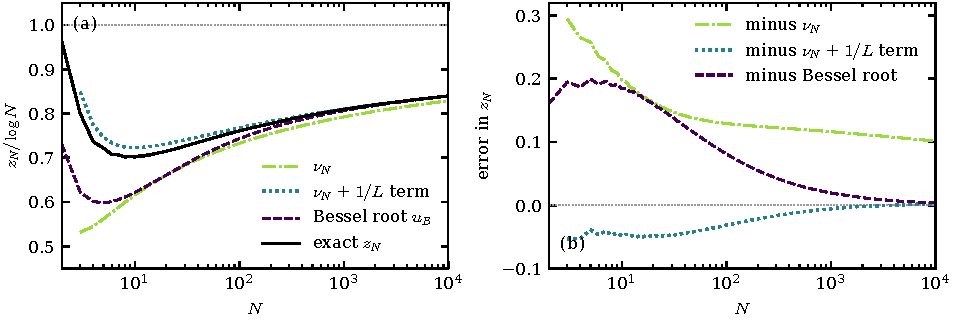
\includegraphics{figures/crossing}
\caption{(a) The scaled crossing $z_N/\log N$ (solid) and the same quantity from the Bessel root
$u_B$ of Theorem~\ref{thm:bessel} (dashed), from $\nu_N$ of \eqref{eq:secondorder} (through the
constant) and from $\nu_N+(\frac14\log L-\frac12c_0+\frac18)/L$ of \eqref{eq:thirdorder} (with the
$1/L$ term). The ratio
tends to $1$ very slowly. (b) The exact $z_N$ minus each approximation.}
\label{fig:crossing}
\end{figure}
